\documentclass{examen}

\begin{document}
\modulo{Planificacion y administracion de redes.}
\pregunta{Observa la red de la figura. Escribe los comandos necesarios para crear VLANs y los subinterfaces asociados de acuerdo a los requisitos siguientes:
\begin{itemize}
	\item{PC0 y PC2 est�n en la VLAN 10. Esta VLAN tendr� la IP 20.10.0.0 con m�scara 255.255.0.0}
	\item{PC5, PC3 y PC4 est�n en la VLAN 20.Esta VLAN tendr� la IP 30.20.0.0 con m�scara 255.255.0.0}
	\item{PC5, PC7 y PC6 est�n en la VLAN 30. Esta VLAN tendr� la IP 40.30.0.0 con m�scara 255.255.0.0}
	\item{Los servidores SMTP y HTTP est�n en su propia VLAN, la 100.Esta VLAN tendr� la IP 8.100.0.0 con m�scara 255.255.0.0}
\end{itemize}

.}{6.5}

\pregunta{Asigna las direcciones IP, m�scaras y gateways que sean necesarios para que todo funcione. Crea tambi�n los comandos necesarios para conseguir lo siguiente:
\begin{itemize}
\item{Se proh�be que las m�quinas del interior tengan acceso al exterior a cualquier servidor HTTP que haya en la red 192.168.10.0/24 .}
\item{Las redes 10.14.0.0/16 y la 10.161.0.0/16 no pueden hacer ping  al SMTP.}
\item{Se prohibe el acceso desde el interior a la red 172.16.0.0/16}
\end{itemize}
.}{3.5}
\begin{figure}
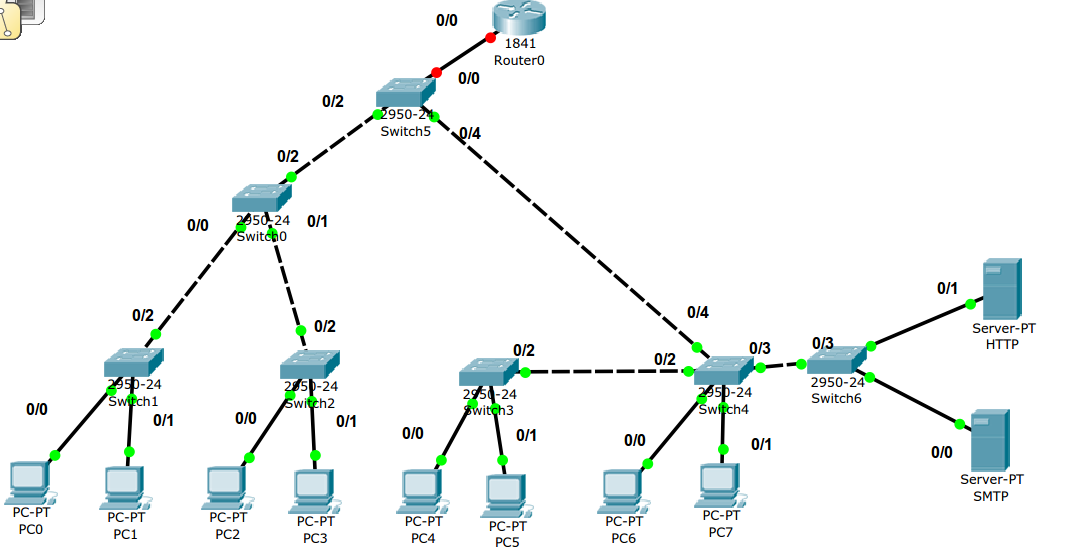
\includegraphics[scale=0.4]{examen-img/vlan.png}
\end{figure}
\end{document}
